% Chapter 1

\chapter{The Application} % Main chapter title

\label{Chapter1} % For referencing the chapter elsewhere, use \ref{Chapter1} 

%----------------------------------------------------------------------------------------

% Define some commands to keep the formatting separated from the content 
\newcommand{\keyword}[1]{\textbf{#1}}
\newcommand{\tabhead}[1]{\textbf{#1}}
\newcommand{\code}[1]{\texttt{#1}}
\newcommand{\file}[1]{\texttt{\bfseries#1}}
\newcommand{\option}[1]{\texttt{\itshape#1}}

%----------------------------------------------------------------------------------------

\section{Overview}
The application consists on 6 services simulating an e-commerce application.

\begin{verbatim}
\begin{figure}
\centering
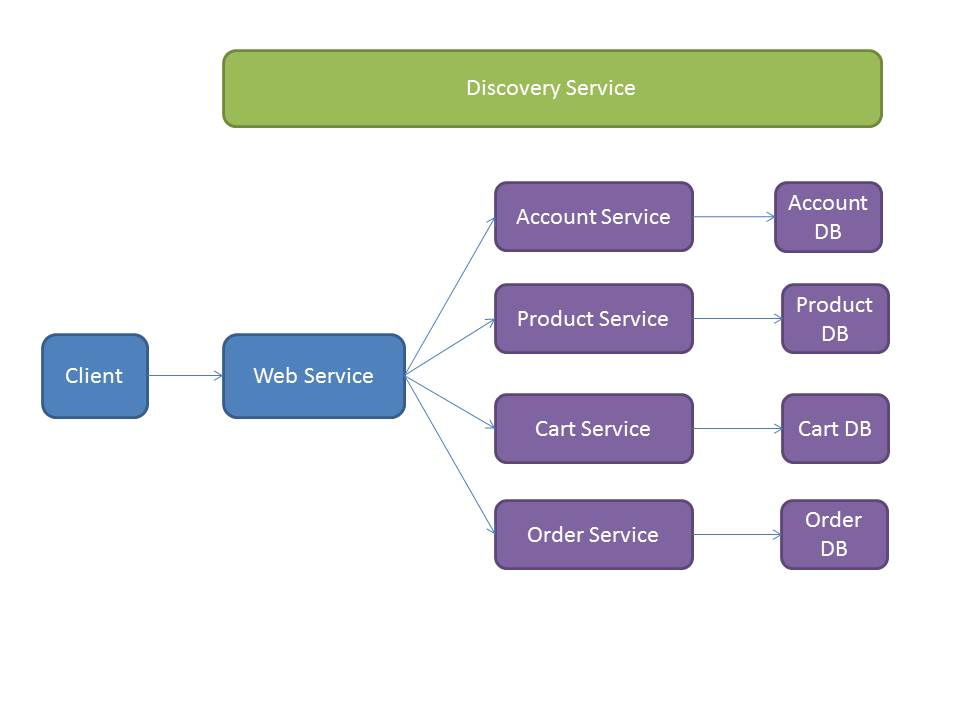
\includegraphics{Figures/Presentation1}
\decoRule
\caption[Block Diagram]{Application block diagram}
\label{fig:Block Diagram}
\end{figure}
\end{verbatim}

The user entry point is the Web Service, from where all the functionality of the application can be accessed. For the sake of simplicity there are no roles defined within the users of the application and thus any request coming from the Web Service is processed by the application.
The Discovery Service is not focussed on functional requirements but it tracks all the available instances of each running service.

What follows is a short description of each one of the services:
\begin{itemize}
\item Web Service: User entry point. Application's functionality is accessed through a REST API 
\item Account Service: Service for managing user accounts. Accounts can be created and deleted.
\item Product Servive: Service that manages the shop product catalogue. Products can be created and deleted.
\item Cart Service: Service that manages the products within the shopping carts.
\item Order Service: Service that manages the carts within the shopping orders.
\item Discovery Service: Discussion of the experimental results
\end{itemize}

Relationships between services as well as the own service behavior is described within the test specification itself and so more details can be found in the next chapter. 

%----------------------------------------------------------------------------------------

\section{Data Model}

The Accounts, Product, Cart and Order Services have each one its own data model:
TODO: Data model classes

%----------------------------------------------------------------------------------------

\section{Assumptions}

All databases start with one test entry:

\begin{itemize}
\item Account: 000000001, "TestUser", 1000
\item Product: ref001, "10", "Simple mouse"
\item Cart: C001, 000000001, ref001
\item Order: O001, C001
\end{itemize}
